% This is samplepaper.tex, a sample chapter demonstrating the
% LLNCS macro package for Springer Computer Science proceedings;
% Version 2.20 of 2017/10/04
%
\documentclass[runningheads]{llncs}

\usepackage[utf8]{inputenc}  % for my name
\usepackage{hyperref}        % hyperlinks
\usepackage{float}           % inline figures

%
\usepackage{graphicx}
% Used for displaying a sample figure. If possible, figure files should
% be included in EPS format.
%
% If you use the hyperref package, please uncomment the following line
% to display URLs in blue roman font according to Springer's eBook style:
\renewcommand\UrlFont{\color{blue}\rmfamily}
\setlength{\intextsep}{1cm}


\begin{document}
%
\title{Information Processing}
\subtitle{Coursework - 6 April 2018}
%
%\titlerunning{Abbreviated paper title}
% If the paper title is too long for the running head, you can set
% an abbreviated paper title here
%
\author{Student number 17113498 \inst{1}}
%
\authorrunning{17113498}
% First names are abbreviated in the running head.
% If there are more than two authors, 'et al.' is used.
%
\institute{University College London, United Kingdom}
%
\maketitle              % typeset the header of the contribution

\section{Tissue Probability Maps}

% Using the 10 tissue segmentations and their associated MR images, create a groupwise mean template and associated tissue probability maps that are representative of this population. Describe the process and justify your choice of transformation model (rigid, affine and/or non-rigid) [15].


Tissue Probability Maps (TPMs) of cerebrospinal fluid (CSF), gray matter (GM), white matter (WM) and background must be generated so that they can be used as spatial priors for tissue segmentation. For that, the group of subjects with an associated label map representing a previous tissue segmentation has been used.


The TPMs are calculated as an average of all the label maps that have been projected to a common space defined by a \textit{template} image. An example of such a template is the one built at the Montreal Neurological Institute (MNI) \cite{evans_3d_1993}. However, for this project a template space has been built iteratively using a groupwise coregistration of all the subjects in the group. All the registrations have been performed using NiftyReg \cite{modat_global_2014}\footnote{The repository containing the Python code used for the experiments (over 2000 lines) and the \LaTeX\ code used to create this report is available online on GitHub, under request to the author.}.


\subsection{Interpolation}
The following interpolation methods have been used when applying a transform to an image:

\subsubsection{TPMs}
Linear interpolation has been used to resample a transformed TPM. This ensures that the values that were between 0 and 1 in the source space remain in that range once interpolated into the target space

\subsubsection{$T_1$-weighted images} To resample anatomical images, sinc interpolation has been used so that the interpolation is smooth. Modifying the original values range is not too relevant

\subsubsection{Label maps} Since the discrete values of the labels must be preserved, nearest-neighbour interpolation has been used to resample the label maps.



\subsection{Similarity measure}
The linear version of NiftyReg (Aladin block-matching algorithm), uses normalised cross-correlation (NCC) as similarity measure. This is appropriate for the registrations performed in this project, since they are all monomodal, i.e. a pairwise linear relationship between image intensities is expected. If registrations were multimodal, e.g. MRI to CT, a different similarity measure as normalised mutual information or joint entropy would be more appropriate.



\subsection{Rigid coregistration}
First, the $T_1$-weighted image of one segmented subject is taken as reference and the rest of the subjects are registered to the reference one by one using rigid registration, i.e. 6 degrees of freedom (DOF) representing translation and rotation. The floating images are resampled to the reference space and averaged in order to generate the initial version of the template image. For visualisation purposes, the label maps have also been transformed to the reference space and the results have been averaged label by label, yielding an initial version of the TPMs. Figure \ref{fig:template-rigid} shows the results of this initial coregistration step.

\begin{figure}
  \centering
  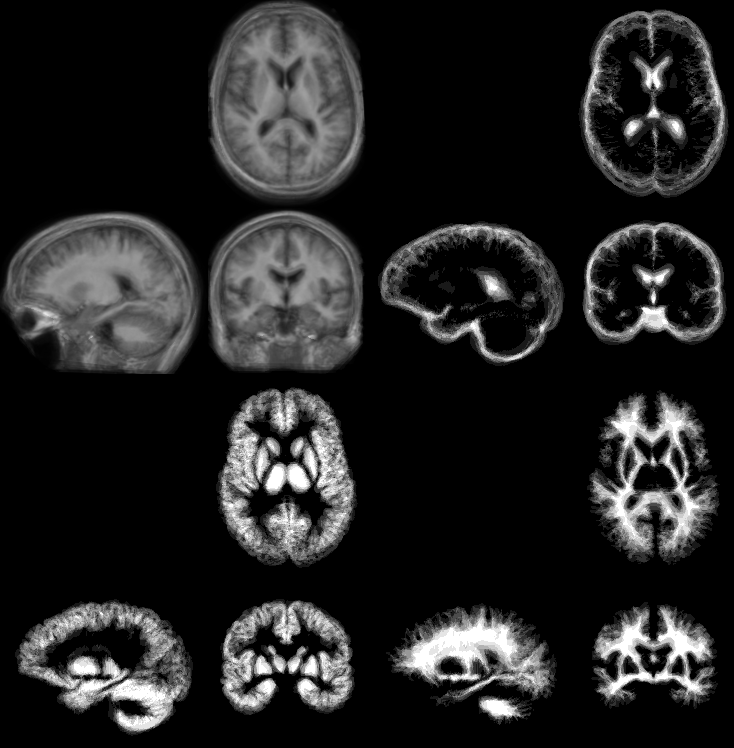
\includegraphics[width=\textwidth]{figures/rigid_template_collage}
  \caption{Results of the rigid coregistration. Top left: mean of the $T_1$-weighted images; top right: TPM of the CSF; bottom left: TPM of the GM; bottom right: TPM of the WM.}
  \label{fig:template-rigid}
\end{figure}

Using only rigid registration for the initial helps reduce the bias of the template. If the first coregistration were performed with using affine registrations (12 DOF representing translation, rotation, shearing and anisotropic scaling), the consecutive iterations would be biased towards the reference image.


\subsection{Iterative affine coregistration}
Once a rigid version of the template is created, it can be used as reference for the following iterations of the coregistration. At each iteration, the transform from the previous step was used for initialisation. This iterative process generated a template image and TPMs that were sharper for each iteration, but did not converge to a final result. Up to 10 iterations, the smoothness reduction stopped being visually perceptible. However, the image seem to diverge towards a sheared version of the template after 10 iterations. Figure \ref{fig:template-sheared} shows a comparison between the template image after 10 and 20 iterations and Figure \ref{fig:template-final} shows the final template after 10 affine iterations.


\begin{figure}
  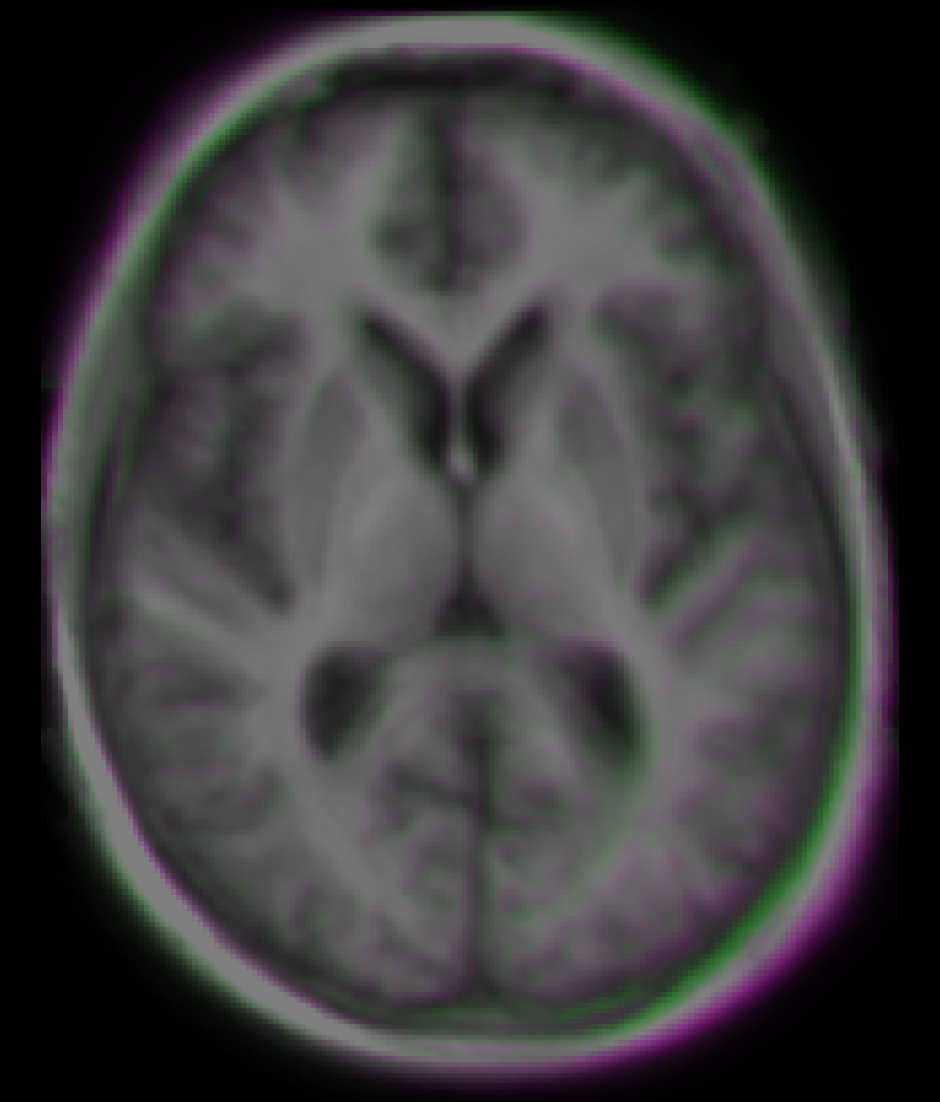
\includegraphics[width=0.5\textwidth]{figures/template_sheared}
  \centering
  \caption{Final template after 10 affine iterations. Top left: mean of the $T_1$-weighted images; top right: TPM of the CSF; bottom left: TPM of the GM; bottom right: TPM of the WM.}
  \label{fig:template-sheared}
\end{figure}


\begin{figure}
  \centering
  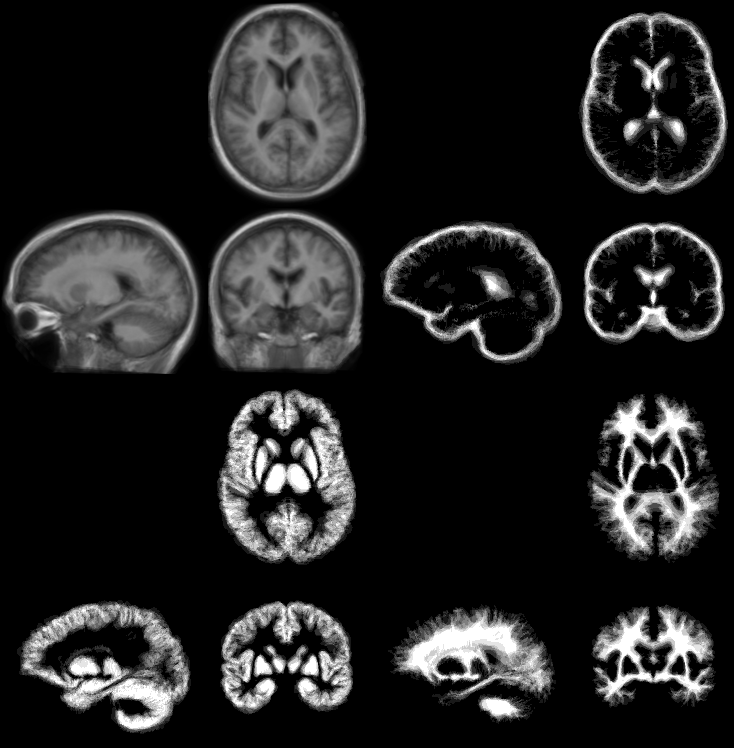
\includegraphics[width=\textwidth]{figures/affine_template_iter_9_collage}
  \centering
  \caption{Template image after 10 affine registration iterations (green) blended with template image after 20 iterations (magenta). The shearing effect is especially visible at the top left and bottom right parts of the image.}
  \label{fig:template-final}
\end{figure}


Moving forward into running coregistration iterations using a free-form registration would result into sharper TPMs, but this might lead to a poorer tissue segmentation, since the priors might not be general enough. For example, if the probability of one voxel being grey matter is close to 0 in the priors that have been propagated to a subject space, that voxel will be missclassified if it actually corresponds to this tissue in that subject image. Early-stopping at affine registration only makes the tissue smoother, capturing a better adaptability of the model to individual cases. Figure \ref{fig:template-std} shows the standard deviation of the final template across the 10 subjects registered to it. The higher variability in the grey matter means that TPMs should be smooth enough to generalise properly. A Gaussian blur image filter may also be used to obtain smoother TPMs, that might generalise even better.

\begin{figure}
  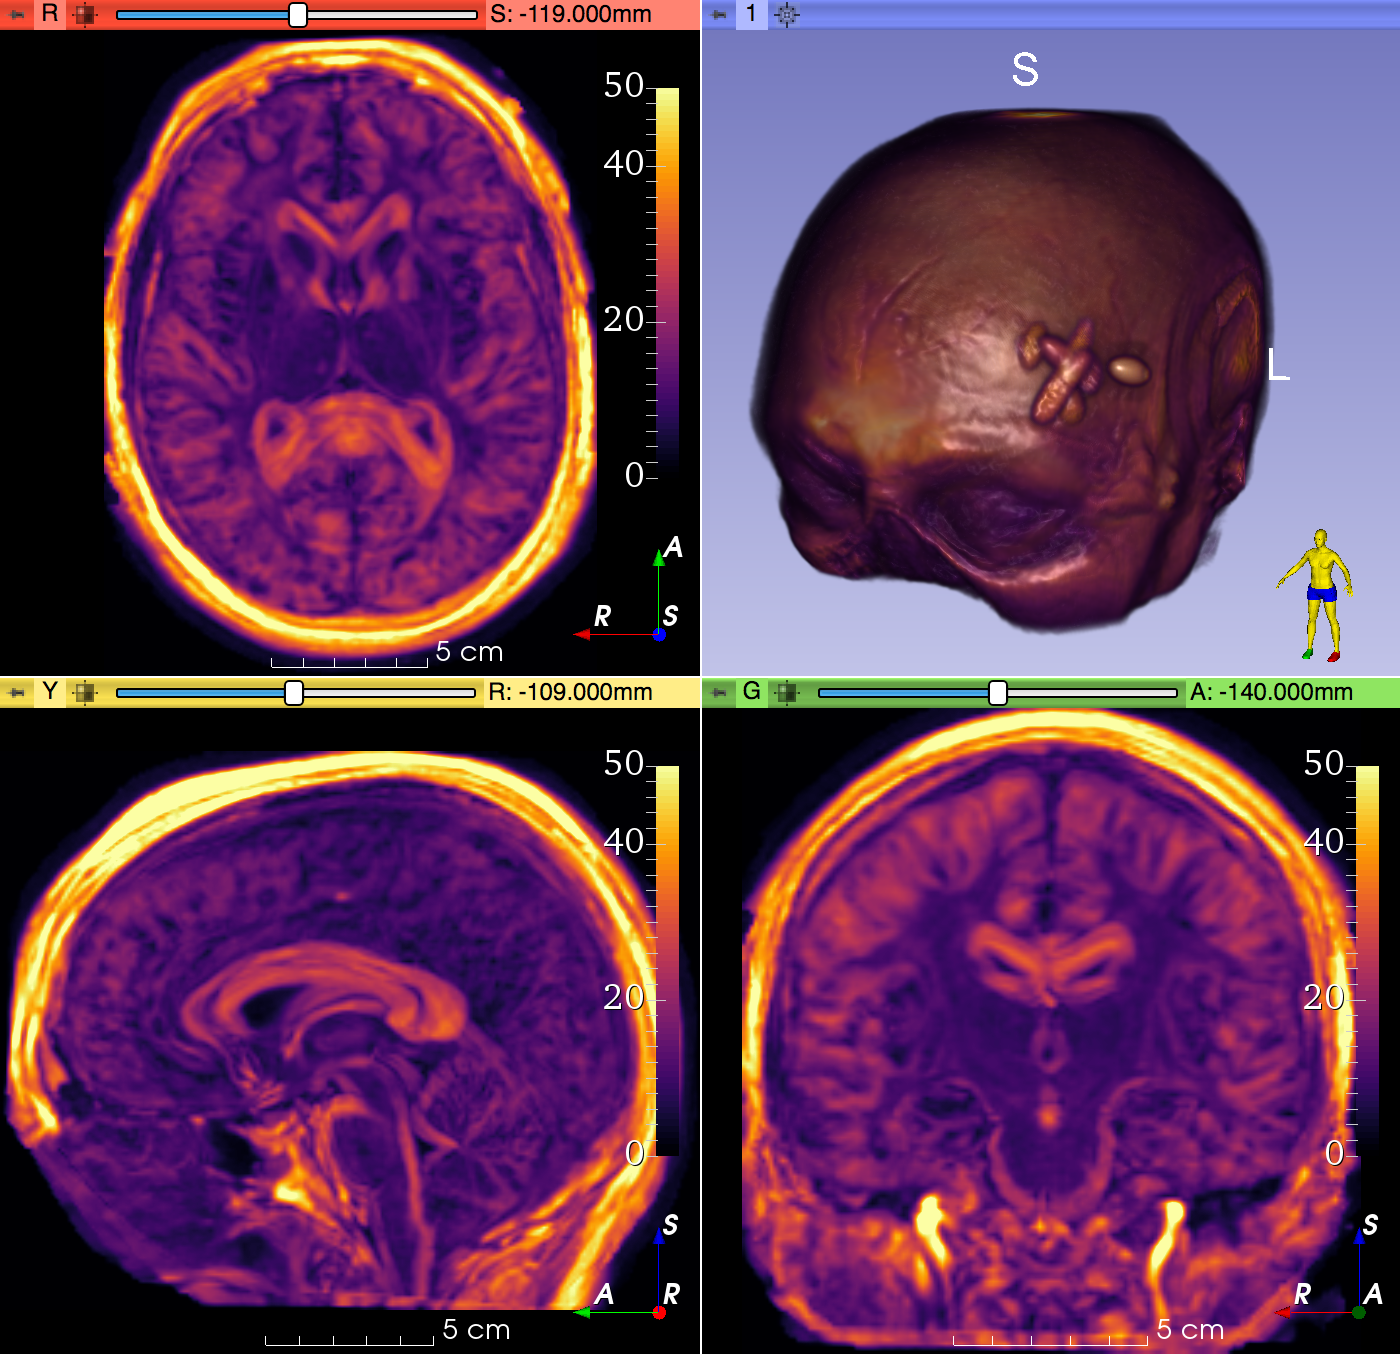
\includegraphics[width=\textwidth]{figures/affine_9_std}
  \centering
  \caption{Standard deviation across the 10 segmented subjects registered to the final template.}
  \label{fig:template-std}
\end{figure}

\section{Tissue segmentation}

% Implement a Gaussian Mixture Model (GMM) to segment the 20 non-segmented MRI brains and optimise your model through an Expectation-Maximisation scheme [15].

\subsection{Expectation-Maximisation}
In order to perform the tissue classification, an Gaussian Mixture Model (GMM) using Expectation-Maximisation (EM) optimisation algorithm has been implemented following \cite{leemput_automated_1999-1}. The initial version that has been developed receives as input the $T_1$-weighted image and the number of classes. The means and variances of the gaussian functions representing each class are initialised randomly, and scaled using the image values:

\begin{equation}
  \mu_k = [\max(y) - \min(y)] R + \min(y)
\end{equation}
and
\begin{equation}
  \sigma^2_k = a R + b [\max(y) - \min(y)]
\end{equation}
where $\mu_k$ is the mean intensity of class $k$, $y$ is the T1 image, $R \sim \mathcal{U}\{0, 1\}$ and $a$ and $b$ are scaling parameters that have been set to 10 and 0.8, respectively.

Once the gaussians parameters have been initialised, the EM loop is run until convergence or until a maximum number of iterations has been reached. The convergence happens when the ratio between the log-likelihood of the current and previous iterations is greater than $1 - \epsilon$, where the convergence threshold $\epsilon$ has been set to $10^{-5}$. The algorithm usually converges around 12 iterations, and the maximum number of iterations has been set to 30. All these parameters are customisable by the user when calling the EM method.

When the EM loop is finished, each voxel is assigned to the class with the highest probability and a label map representing the automatic segmentation is saved. Figure \ref{fig:em-first} shows the results of a segmentation. Dice scores are computed comparing each label with the provided label maps, that are used as ground truth. Since no spatial information is used, the algorithm has assigned voxels outside the brain to be brain tissue, and some voxels are isolated within a different class, which is is not plausible anatomically. Adding TPMs as priors and using Markov random field (MRF) smoothing is necessary to produce a more realistic output.

\begin{figure}
  \centering
  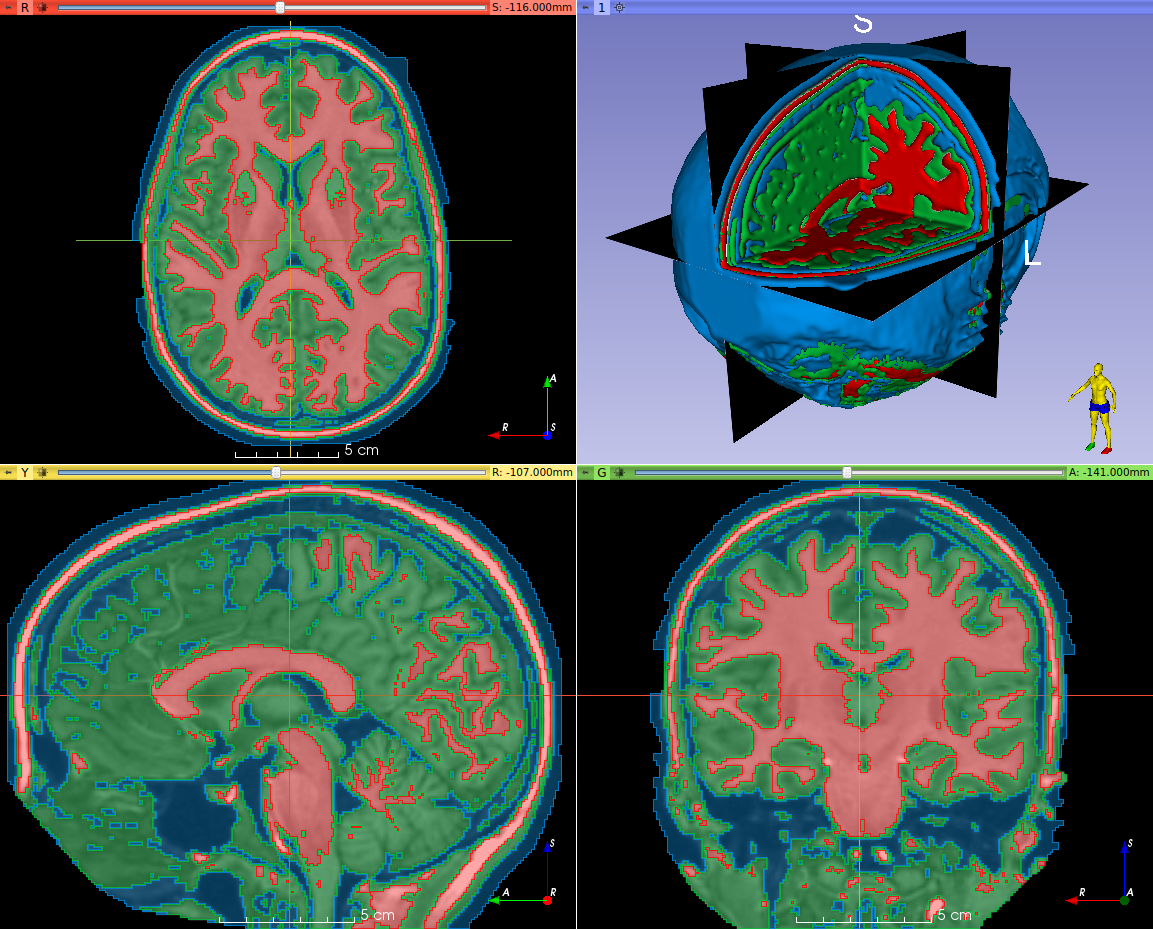
\includegraphics[width=\textwidth]{figures/em_first}
  \caption{Results of an automatic EM segmentation. Approximate classes are: blue - CSF; green - GM; green - WM.}
  \label{fig:em-first}
\end{figure}

The uncertainty of the algorithm assigning a voxel $i$ to a class can be measured as $u_i = 1 - \sigma_i$. Figure \ref{fig:experiment-a} shows another representation of the segmentation of this experiment (named A), including the uncertainty image. The most certain zones are the background and the inner parts of the WM, while the most uncertain ones are the interfaces between different tissues. There is however a high uncertainty in most parts of the head.

\begin{figure}
  \centering
  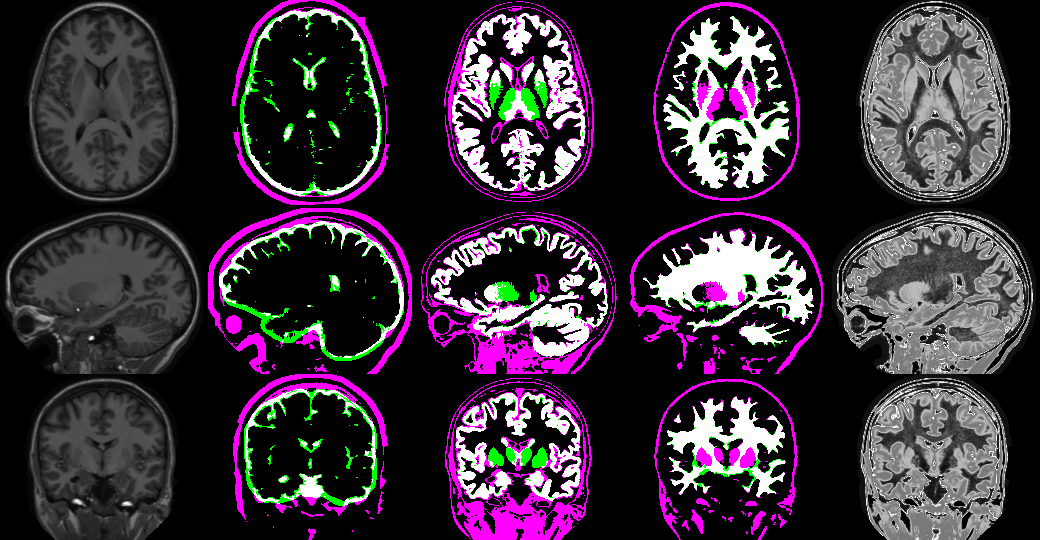
\includegraphics[width=\textwidth]{figures/experiment_a}
  \caption{Results of experiment A: EM segmentation. From left to right: $T_1$-weighted image; CSF, GM and WM segmentations; uncertainty. In the segmentations, white voxels are TP, black voxels are TN, green voxels are FN and magenta voxels are FP.}
  \label{fig:experiment-a}
\end{figure}

Some observations from the segmentation images can be made:
\begin{itemize}
  \item Dark parts outside the brain like the eyes have been incorrectly classified as CSF. Also, all the heads seem to have been segmented by Otsu-thresholding, closing, dilation and masking. This creates a noisy zone around the head which corresponds to the original image background. The masked out part of the images is totally black, therefore those voxels are all assigned to the background class in this experiment (the background class always has $\mu = 0$ and $\sigma^2 = 0$)
  \item GM structures with high intensity like the lateral part of the thalamus or the posterior part of the putamen have been incorrectly classified as WM. Again, a lot of tissue outside the brain has been assigned to these classes, given that no spatial a priori information has been provided.
\end{itemize}



% Use image registration to propagate the previously generated tissue probability maps into the space of the non-segmented brain MRIs. This can be achieved by registering the groupwise mean template to the non- segmented brain and then applying the obtained transformation to the probability maps.
% Use then the propagated probability maps as a priori information in your GMM [10]. If you did not complete the previous section, you may use the provided prior files.

\subsection{Initialisation using tissue priors}
The previously generated TPMs can be used as spatial priors within the bayesian framework implemented in the GMM. First, they must be propagated to the subject's space. For that, the template image is non-linearly registered to the subject's $T_1$-weighted MRI and the resulting transform is applied to the TPMs. Using this spatial a priori leads to better qualitative and quantitative results, as shown in Figure~\ref{fig:experiment-b}, which shows the results of experiment B. Also, the algorithm runs faster thans to an initialisation of the Gaussians parameters using the priors. Furthermore, the label maps are consistently sorted, in contrast to experiment A, where the parameters are randomly computed.

\begin{figure}
  \centering
  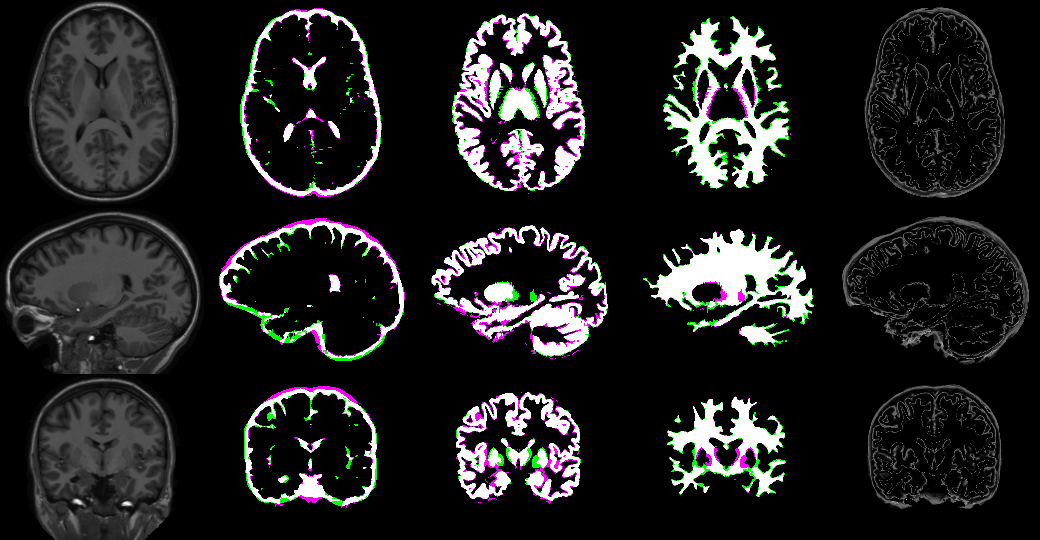
\includegraphics[width=\textwidth]{figures/experiment_b}
  \caption{Results of experiment B: EM segmentation using spatial priors. From left to right: $T_1$-weighted image; CSF, GM and WM segmentations; uncertainty. In the segmentations, white voxels are TP, black voxels are TN, green voxels are FN and magenta voxels are FP.}
  \label{fig:experiment-b}
\end{figure}

Figure \ref{fig:experiment-b} shows that results using the TPMs as spatial priors are qualitatively better:
\begin{itemize}
  \item All the tissue that is far from the brain has been correctly classified as background
  \item Some false negatives in the CSF seem to have been misclassified in the provided segmentation used as ground truth, as shown in Figure~\ref{manual-wrong}. Most of the false negatives are in dark tissue near the ground-truth CSF
  \item Most of the wrong values of GM and WM are in the interfaces between both tissues, but some of the voxels are isolated
  \item The uncertainty is higher around the CSF and on the interfaces between different tissues, which is coherent to the segmentation results.
\end{itemize}


\begin{figure}
  \centering
  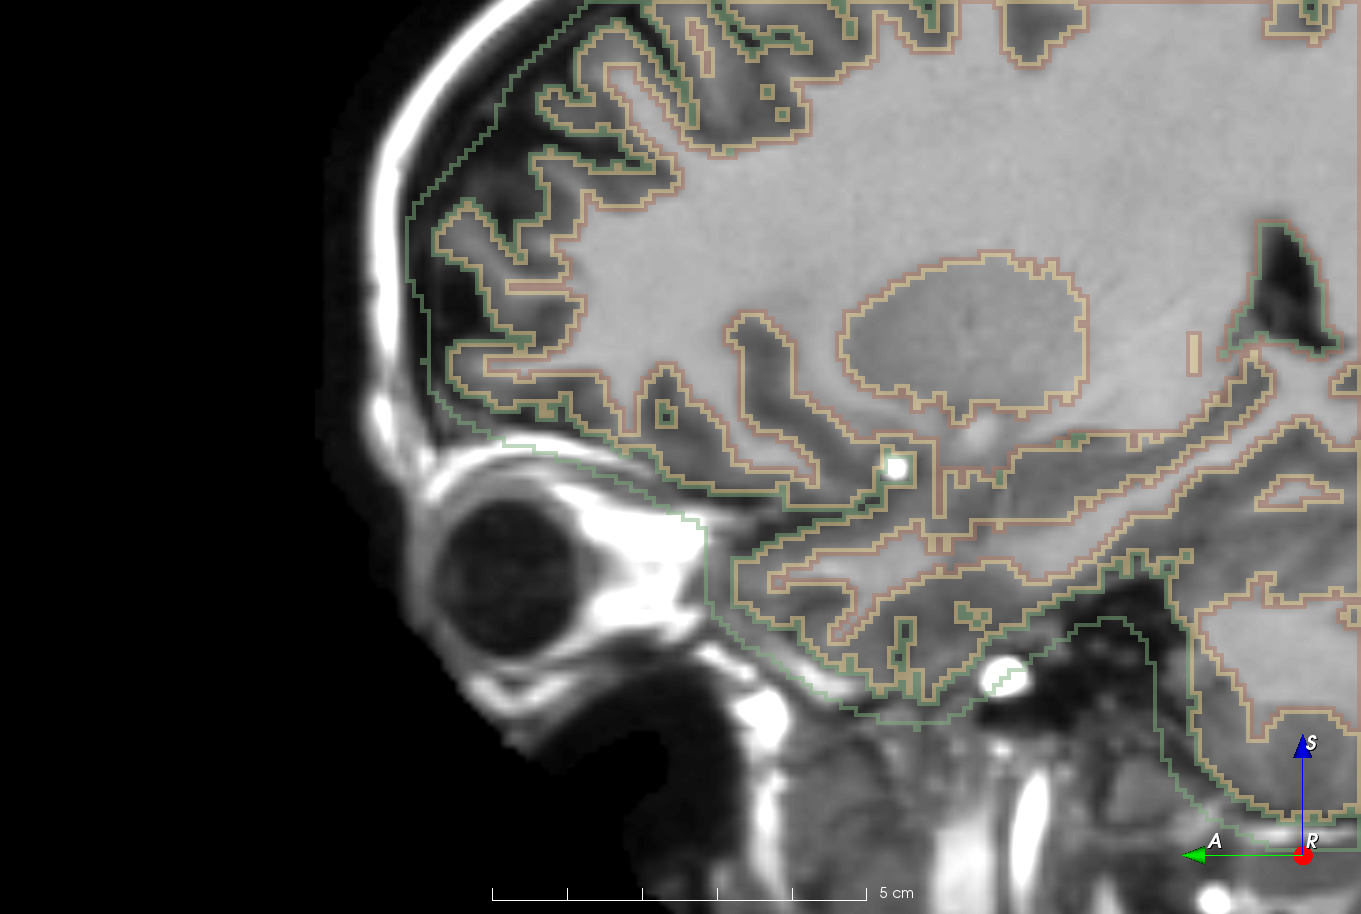
\includegraphics[width=\textwidth]{figures/priors_manual_wrong}
  \caption{Detail of the ground truth segmentation. Tissue around the eye has been incorrectly classified as CSF.}
  \label{fig:manual-wrong}
\end{figure}




\subsubsection{TPMs propagation}

TODO
% TODO: explain choice of reg_f3d bending energy
% Since the TPMs and the template have been built with linear registrations only, the same logic must be applied while propagating them. This means that the free-form registration must be flexible enough to adapt to the subject's anatomy while producing a smooth resampled TPM that ensures a certain generalisability.

% TODO: show displacement field and jacobian



\subsection{Regularisation with Markov random fields}

% Embed a Markov random field into your segmentation framework to introduce a spatial smoothness term in the label estimation process [10].

A voxel with different intensity than all its closest neighbors may be incorrectly classified if its priors for multiple classes are close. This leads to isolated voxels, e.g. voxels of GM in the middle of the WM. Embedding a Markov random field (MRF) into the segmentation helps smoothing the labels, potentially improving the anatomical plausibility of the segmentation. More specifically, a sixth-order Gibbs Random Field has been implemented \cite{leemput_automated_1999-1}. The probabilities array is multiplied by $e^{- \beta U_{MRF}(.)}$, where $U_{MRF}$ is the energy function of the MRF and $\beta$ is a weighting parameter used to control the effect of the MRF on the segmentation. Figure \ref{fig:experiment-c} shows the results of a segmentations that include MRF smoothing for $\beta = 0.2$. Qualitatively, it can be seen that some of the voxels inside the brain that had been classified as CSF without regularisation are now corractly classified. Using a higher value of $\beta$ helps removing isolated voxels, but it comes with a cost of misclassifying many voxels around the sulci, as will be shown later.

\begin{figure}
  \centering
  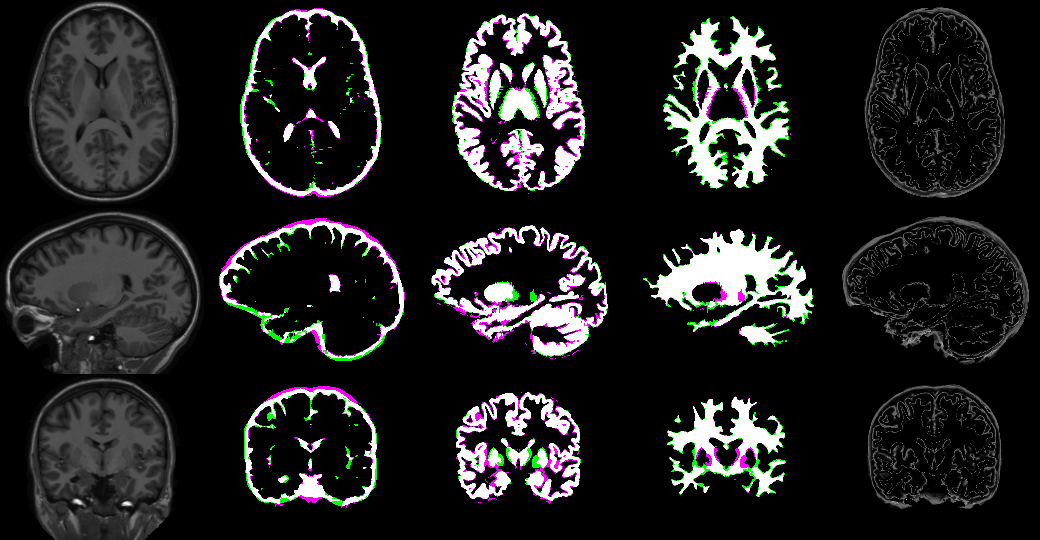
\includegraphics[width=\textwidth]{figures/experiment_b}
  \caption{Results of experiment C: EM segmentation using spatial priors and MRF regularisation. From left to right: $T_1$-weighted image; CSF, GM and WM segmentations; uncertainty. In the segmentations, white voxels are TP, black voxels are TN, green voxels are FN and magenta voxels are FP.}
  \label{fig:experiment-c}
\end{figure}



\subsection{Bias field correction}

% MRI acquisition usually suffers from intensity non-uniformity (INU), improve the robustness of your GMM framework to INU by adding a bias field correction component to the probabilistic model [5].

Since MRI acquisition usually suffers from intensity non-uniformity (INU) due to inhomogeneities in the static magnetic field of the MR scanner, a bias field correction component has been also embedded into the segmentation framework. The bias field is modelled using three-dimensional polynomials whose coefficients are computed using a weighted least-squares fit, as in \cite{leemput_automated_1999}. The implemented algorithm can use polynomial orders from 0 to 3.

The computed bias field can be saved after the segmentation process, as shown in Figure \ref{fig:bias-field}. The extracted bias fields from most images look similar: bright in the head and darker outside it. This might be due to two reasons:
\begin{enumerate}
  \item The images used for this project have already been preprocessed to remove some of the intrinsic bias field artefact
  \item The algorithm tries to remove bias from the voxels classified as background, which is not useful in this case. A possible extension of the classification algorithm would be using only the foreground voxels for the bias field correction step.
\end{enumerate}
Therefore, very small changes in the quality of the segmentation are expected when using the INU correction step. Figure~\ref{fig:experiment-d} shows the result of Experiment D, using polynomials of order $n = 2$.

\begin{figure}
  \centering
  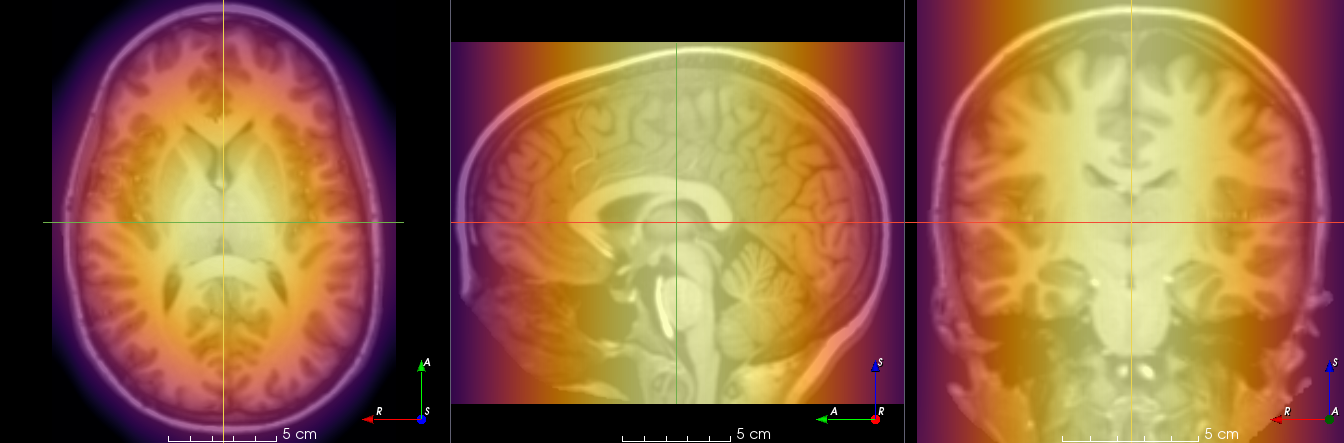
\includegraphics[width=\textwidth]{figures/bias_field}
  \caption{Estimated bias field superimposed on the $T_1$-weighted image. Higher intensity represents larger bias.}
  \label{fig:bias-field}
\end{figure}

\begin{figure}
  \centering
  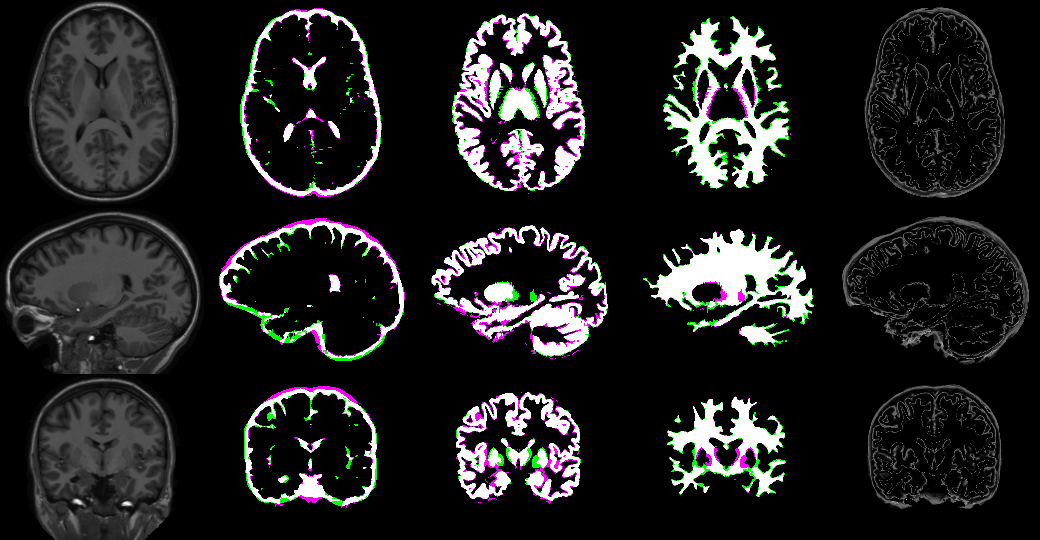
\includegraphics[width=\textwidth]{figures/experiment_b}
  \caption{Results of experiment D: EM segmentation using spatial priors, MRF regularisation and INU correction. From left to right: $T_1$-weighted image; CSF, GM and WM segmentations; uncertainty. In the segmentations, white voxels are TP, black voxels are TN, green voxels are FN and magenta voxels are FP.}
  \label{fig:experiment-d}
\end{figure}


\subsection{Stronger regularisation}
Experiment E consisted on segmenting using $\beta = 2$, which produces a smoother segmentation. Figure~\ref{fig:experiment-e} shows the results.

\begin{figure}
  \centering
  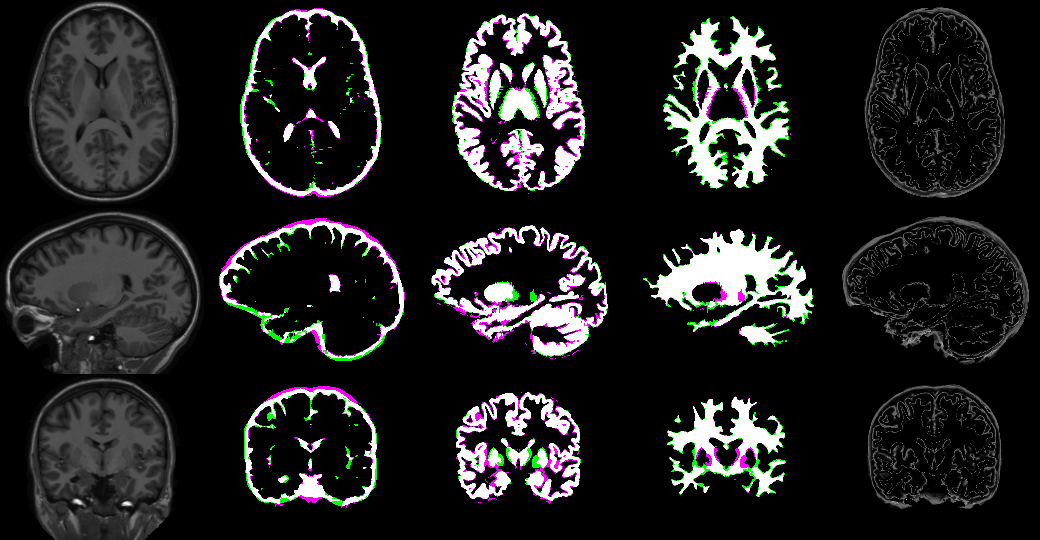
\includegraphics[width=\textwidth]{figures/experiment_b}
  \caption{Results of experiment E: EM segmentation using spatial priors, strong MRF regularisation and INU correction. From left to right: $T_1$-weighted image; CSF, GM and WM segmentations; uncertainty. In the segmentations, white voxels are TP, black voxels are TN, green voxels are FN and magenta voxels are FP.}
  \label{fig:experiment-e}
\end{figure}



\subsection{Quantitative comparison}
The automatic segmentations and the ground truth can be compared quantitatively using a similarity metric like the Dice score. Figure~\ref{fig:experiments} shows that embedding the anatomical priors into the segmentation framework (B) improves the results dramatically compared to the initial algorithm results (A); a small regularisation has almost no effect on the score (C); the INU correction improves it slightly (D); and using too much regularisation leads to less accurate results (E).

\begin{figure}
  \centering
  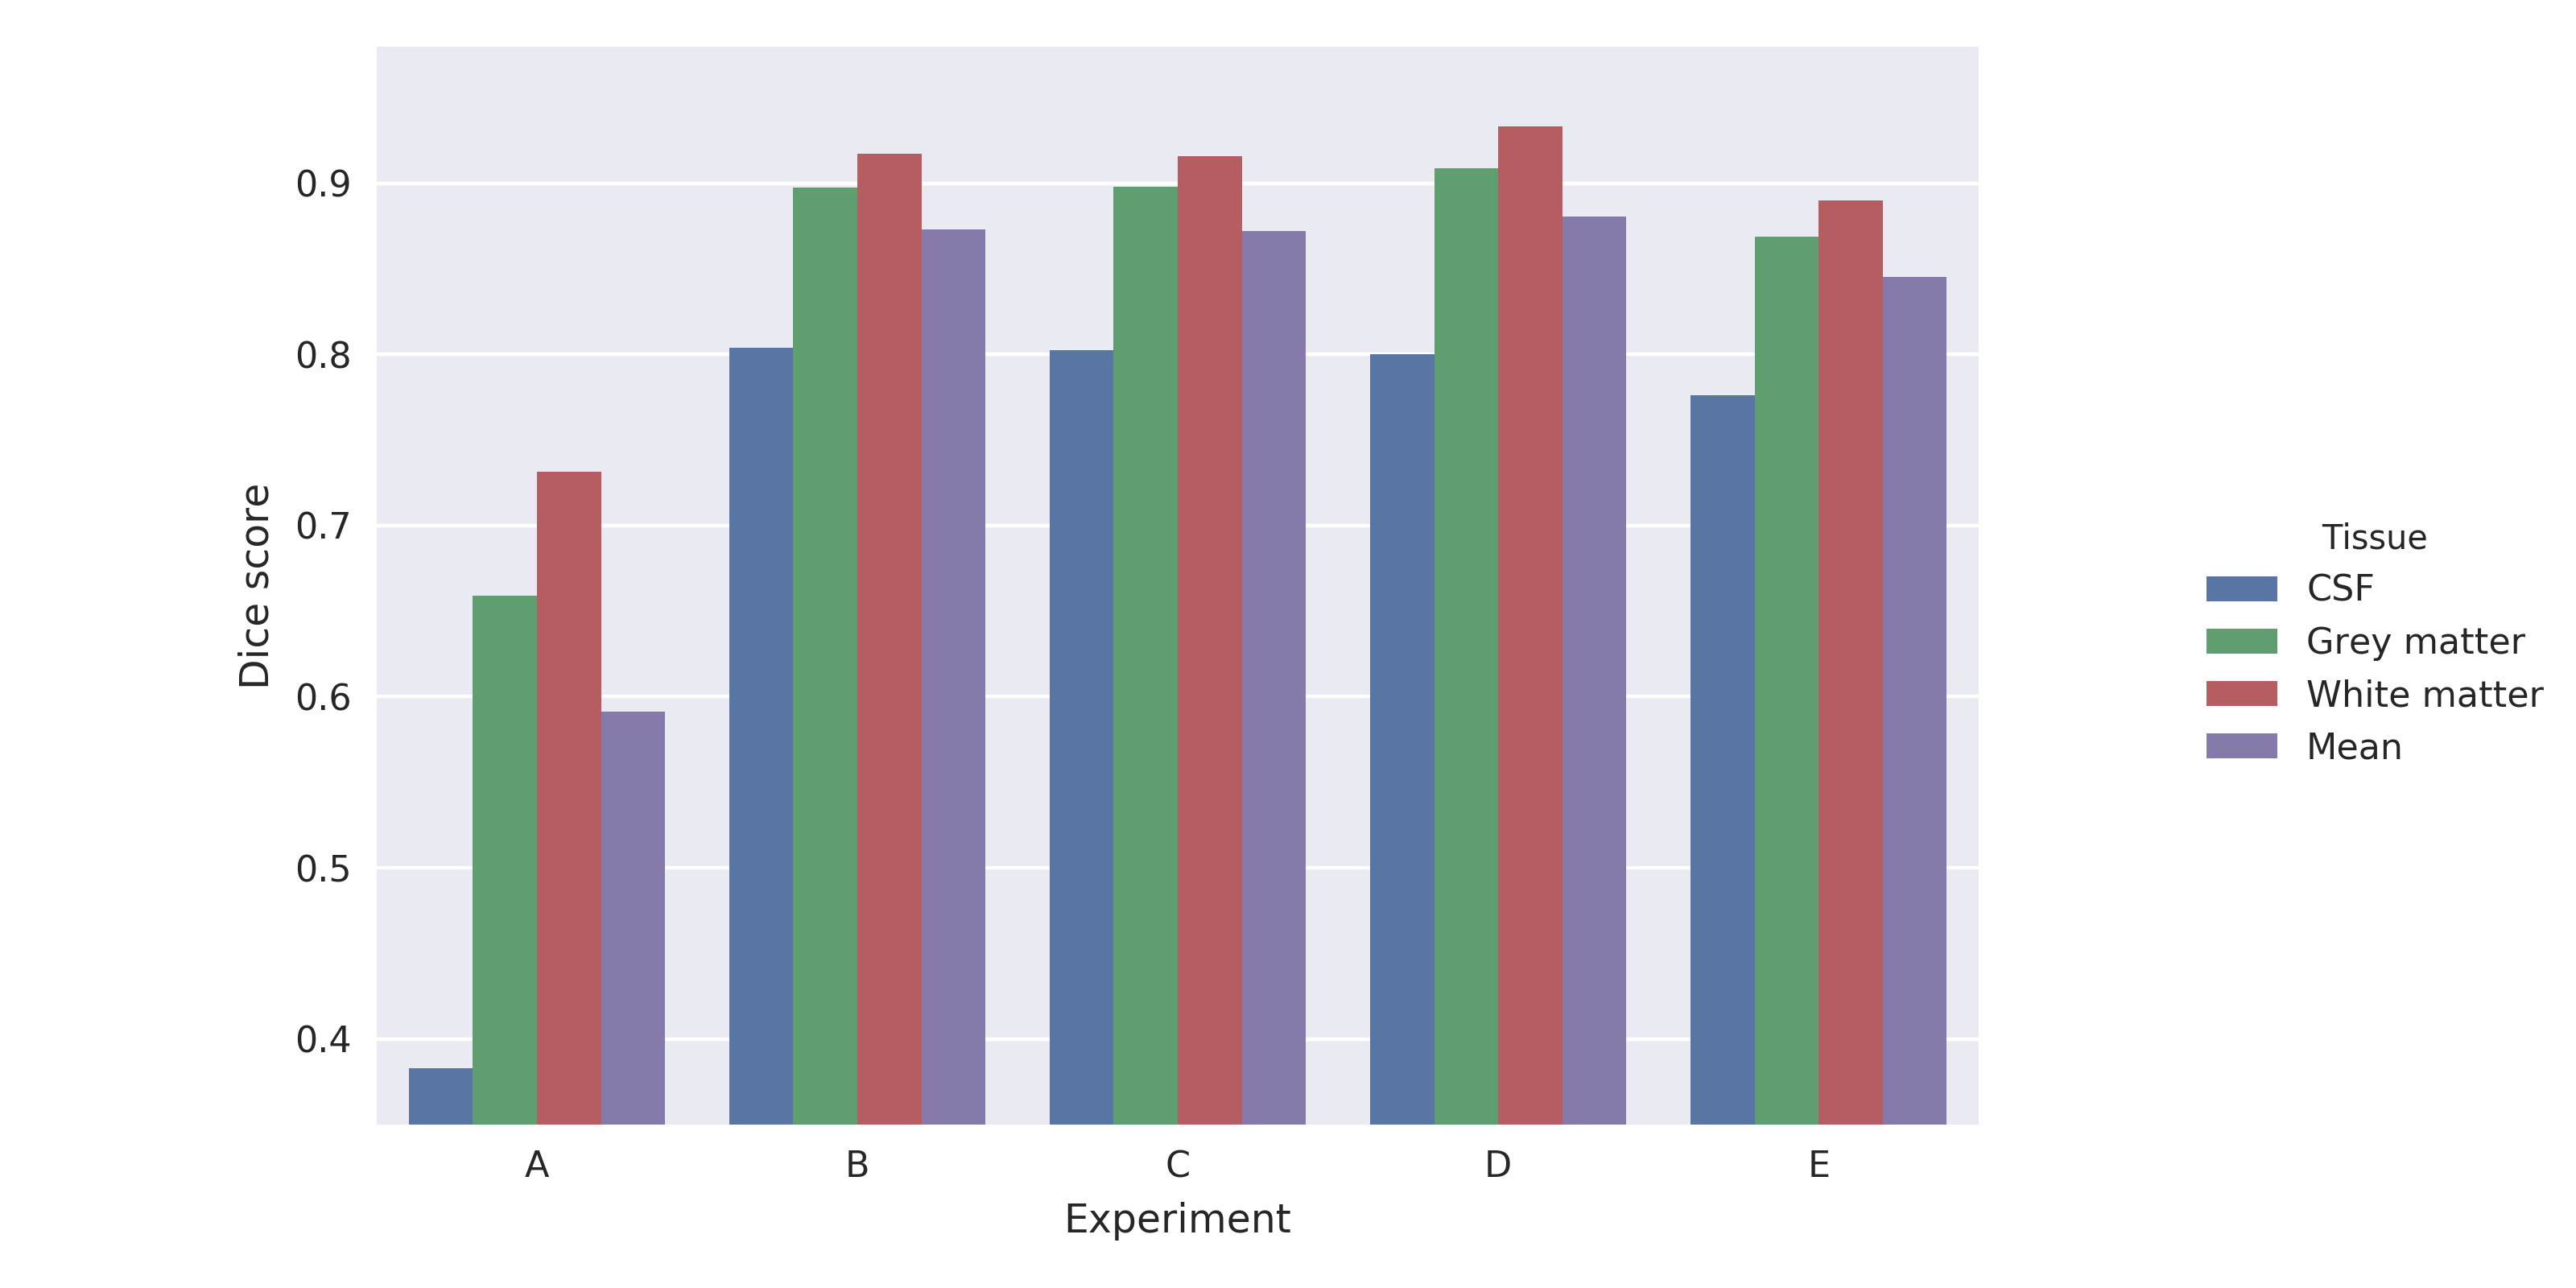
\includegraphics[width=\textwidth]{figures/experiments_dices_bars}
  \caption{Dice scores for the five experiments run on the first subject. A: initial algorithm; B: priors added; C: MRF regularisation added; D: INU correction added; E: effect of a regularisation using a value $\beta$ that is too high.}
  \label{fig:experiments}
\end{figure}




\subsection{Parameters optimisation}

% Use one already segmented images to optimise your implementation parameters (e.g. INU complexity, MRF beta term) [10].

A regular parameter grid has been generated in order to sample the parameter space looking for the best Dice scores, using the first segmented subject. The polinomial orders were 0, 1, 2 and 3 and 8 values of $\beta$ in a logarithmic space from 0.01 to 2 have been sampled. Figure \ref{fig:params-optimisation} shows the results of this parameters search. Interpolating the Dice scores using bicubic interpolation shows that a good choice for the polynomials order is 2 or 3, while $\beta$ should be lower than 1 for good scores. Following segmentation experiments have been performed with polynomial order $n = 2$ and MRF weight $\beta = 0.2$.



\begin{figure}
  \centering
  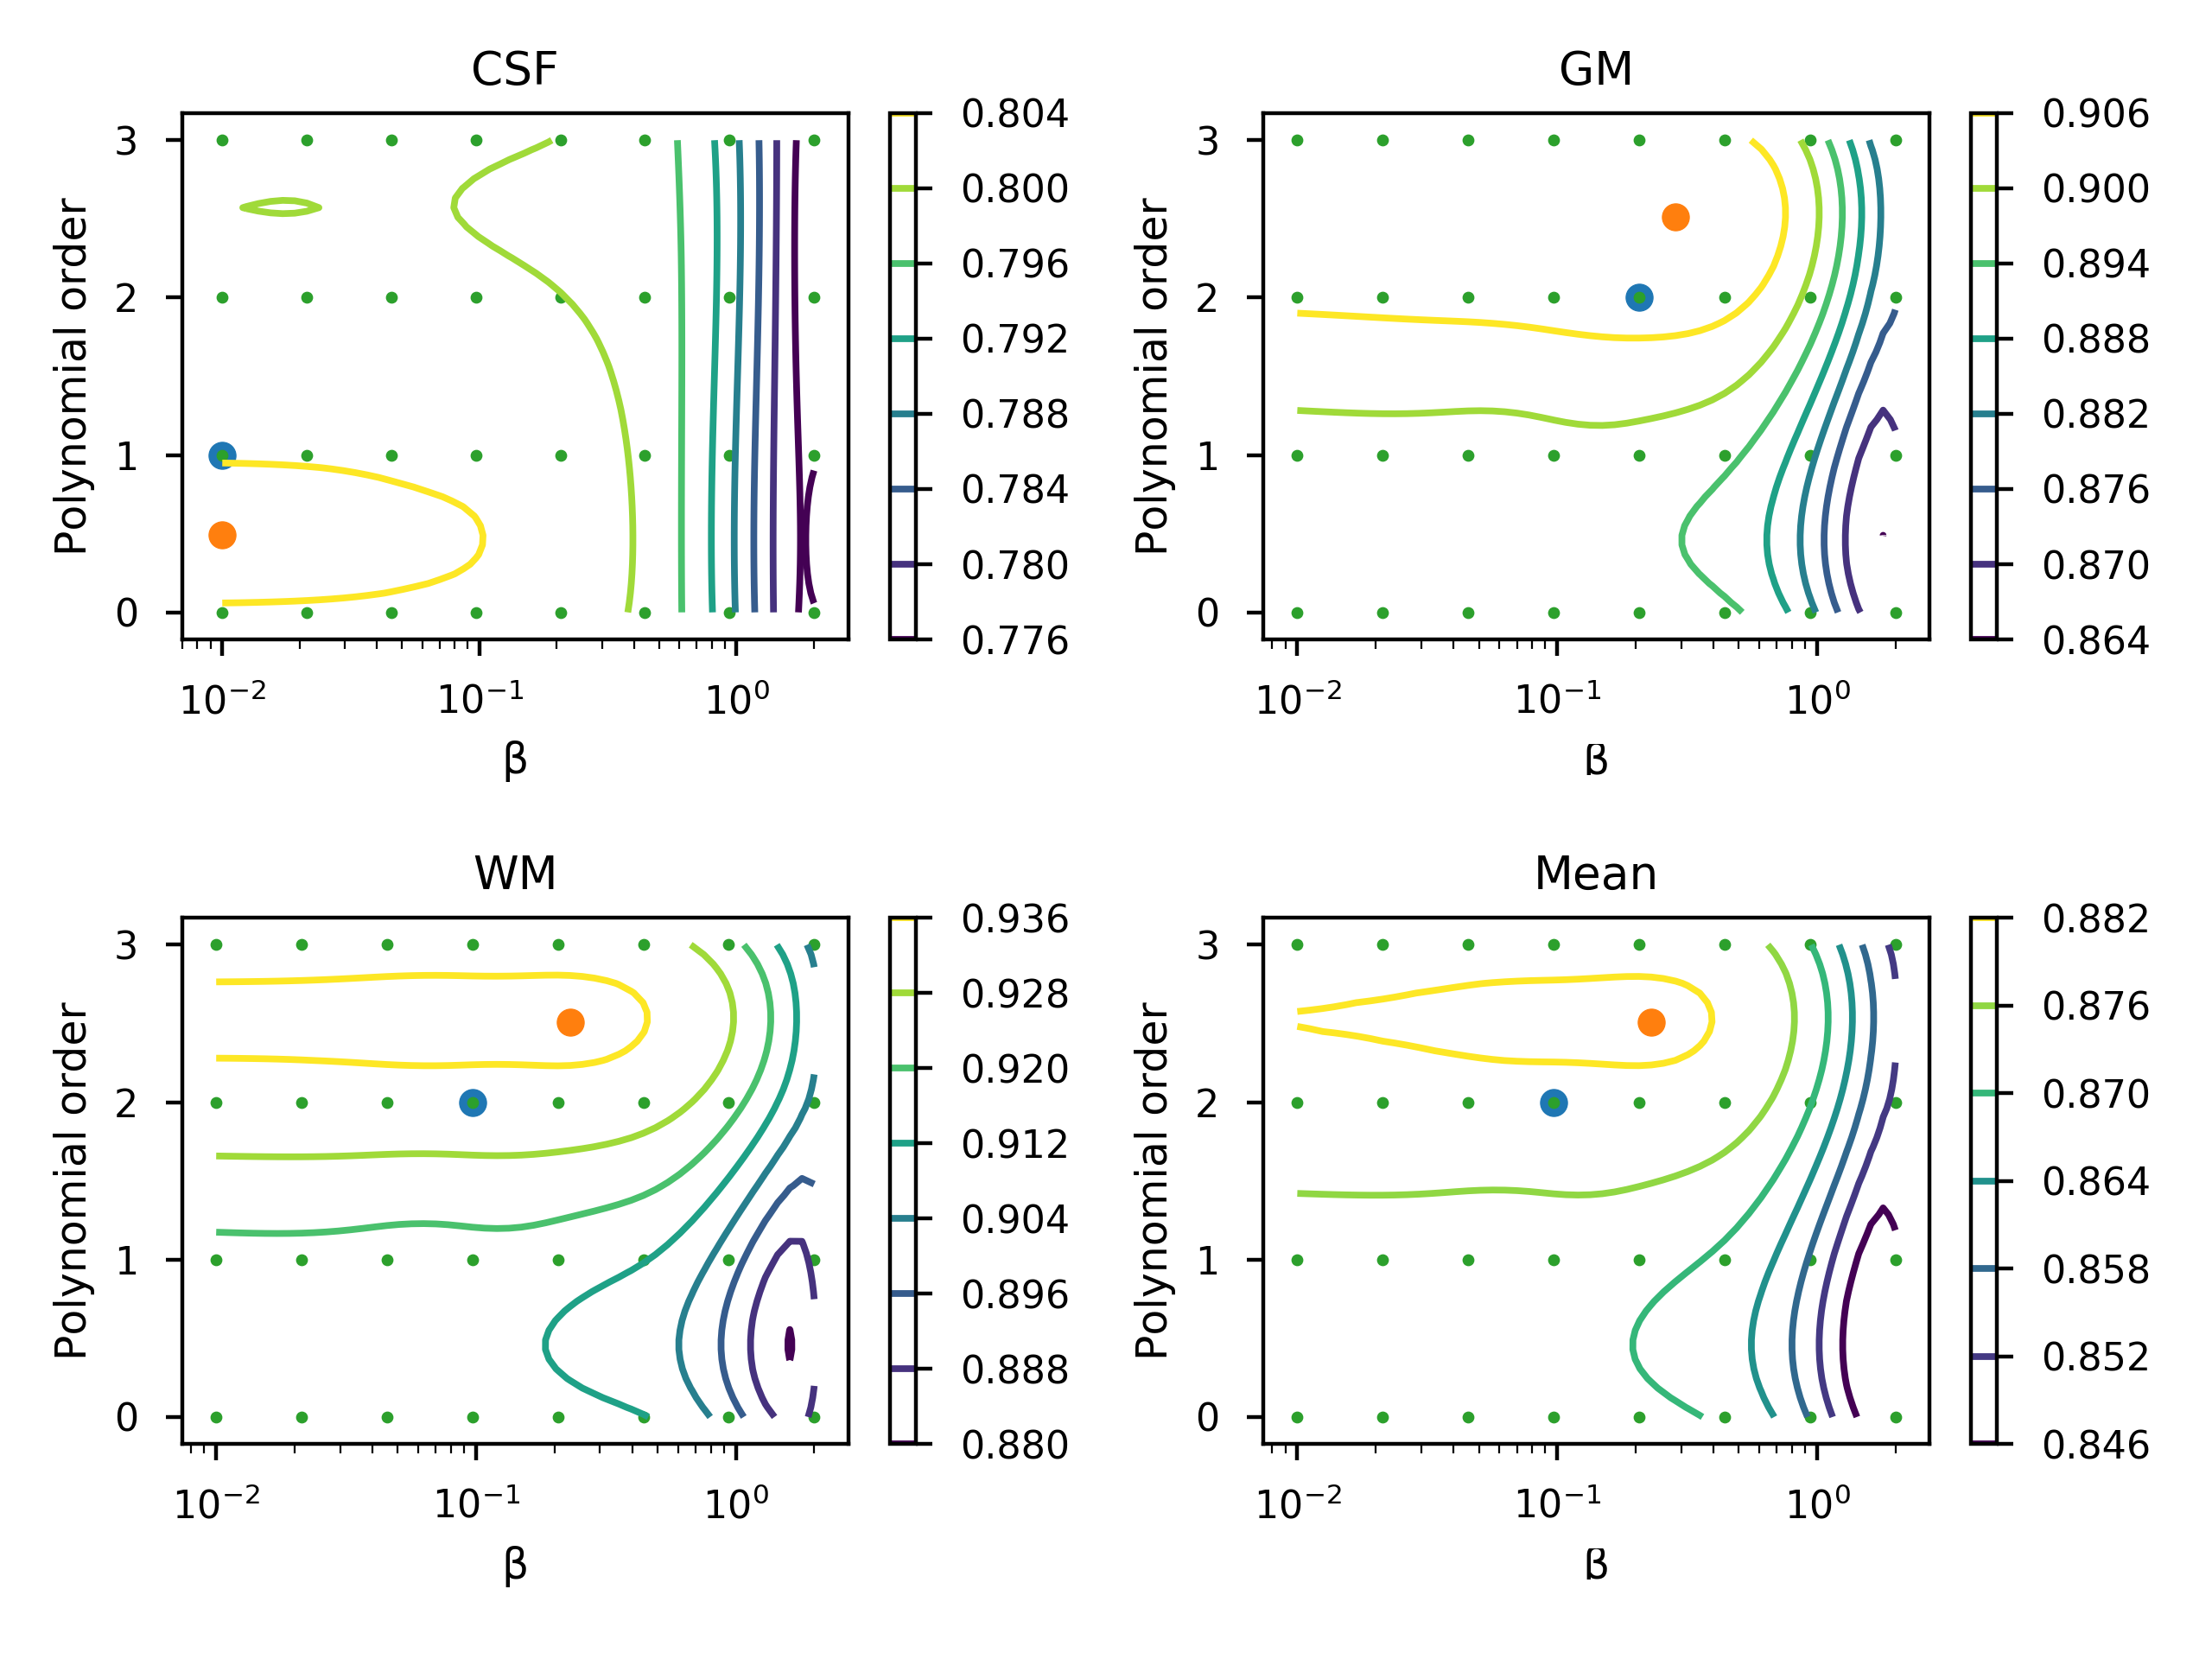
\includegraphics[width=\textwidth]{figures/parameters_dices}
  \caption{Contour plots representing Dice scores for the different parameters. The contours are isolines of the sampled scores interpolated using bicubic interpolation. Green dots represented sampled points; blue dots are the highest sampled Dice score; orange dots are the highest interpolated Dice score.}
  \label{fig:params-optimisation}
\end{figure}


% By choosing these parameters, bias can be introduced in the optimisation. Describe one potential bias and propose a solution to avoid it [5]?

Optimising the segmentation parameters using only data from one subject leads to an overfit towards this subject, as shown in Figure \ref{fig:dices-bars}. If all the subjects were used for the parameters optimisation, the mean Dice score for the whole group would probably be higher.

\begin{figure}
  \centering
  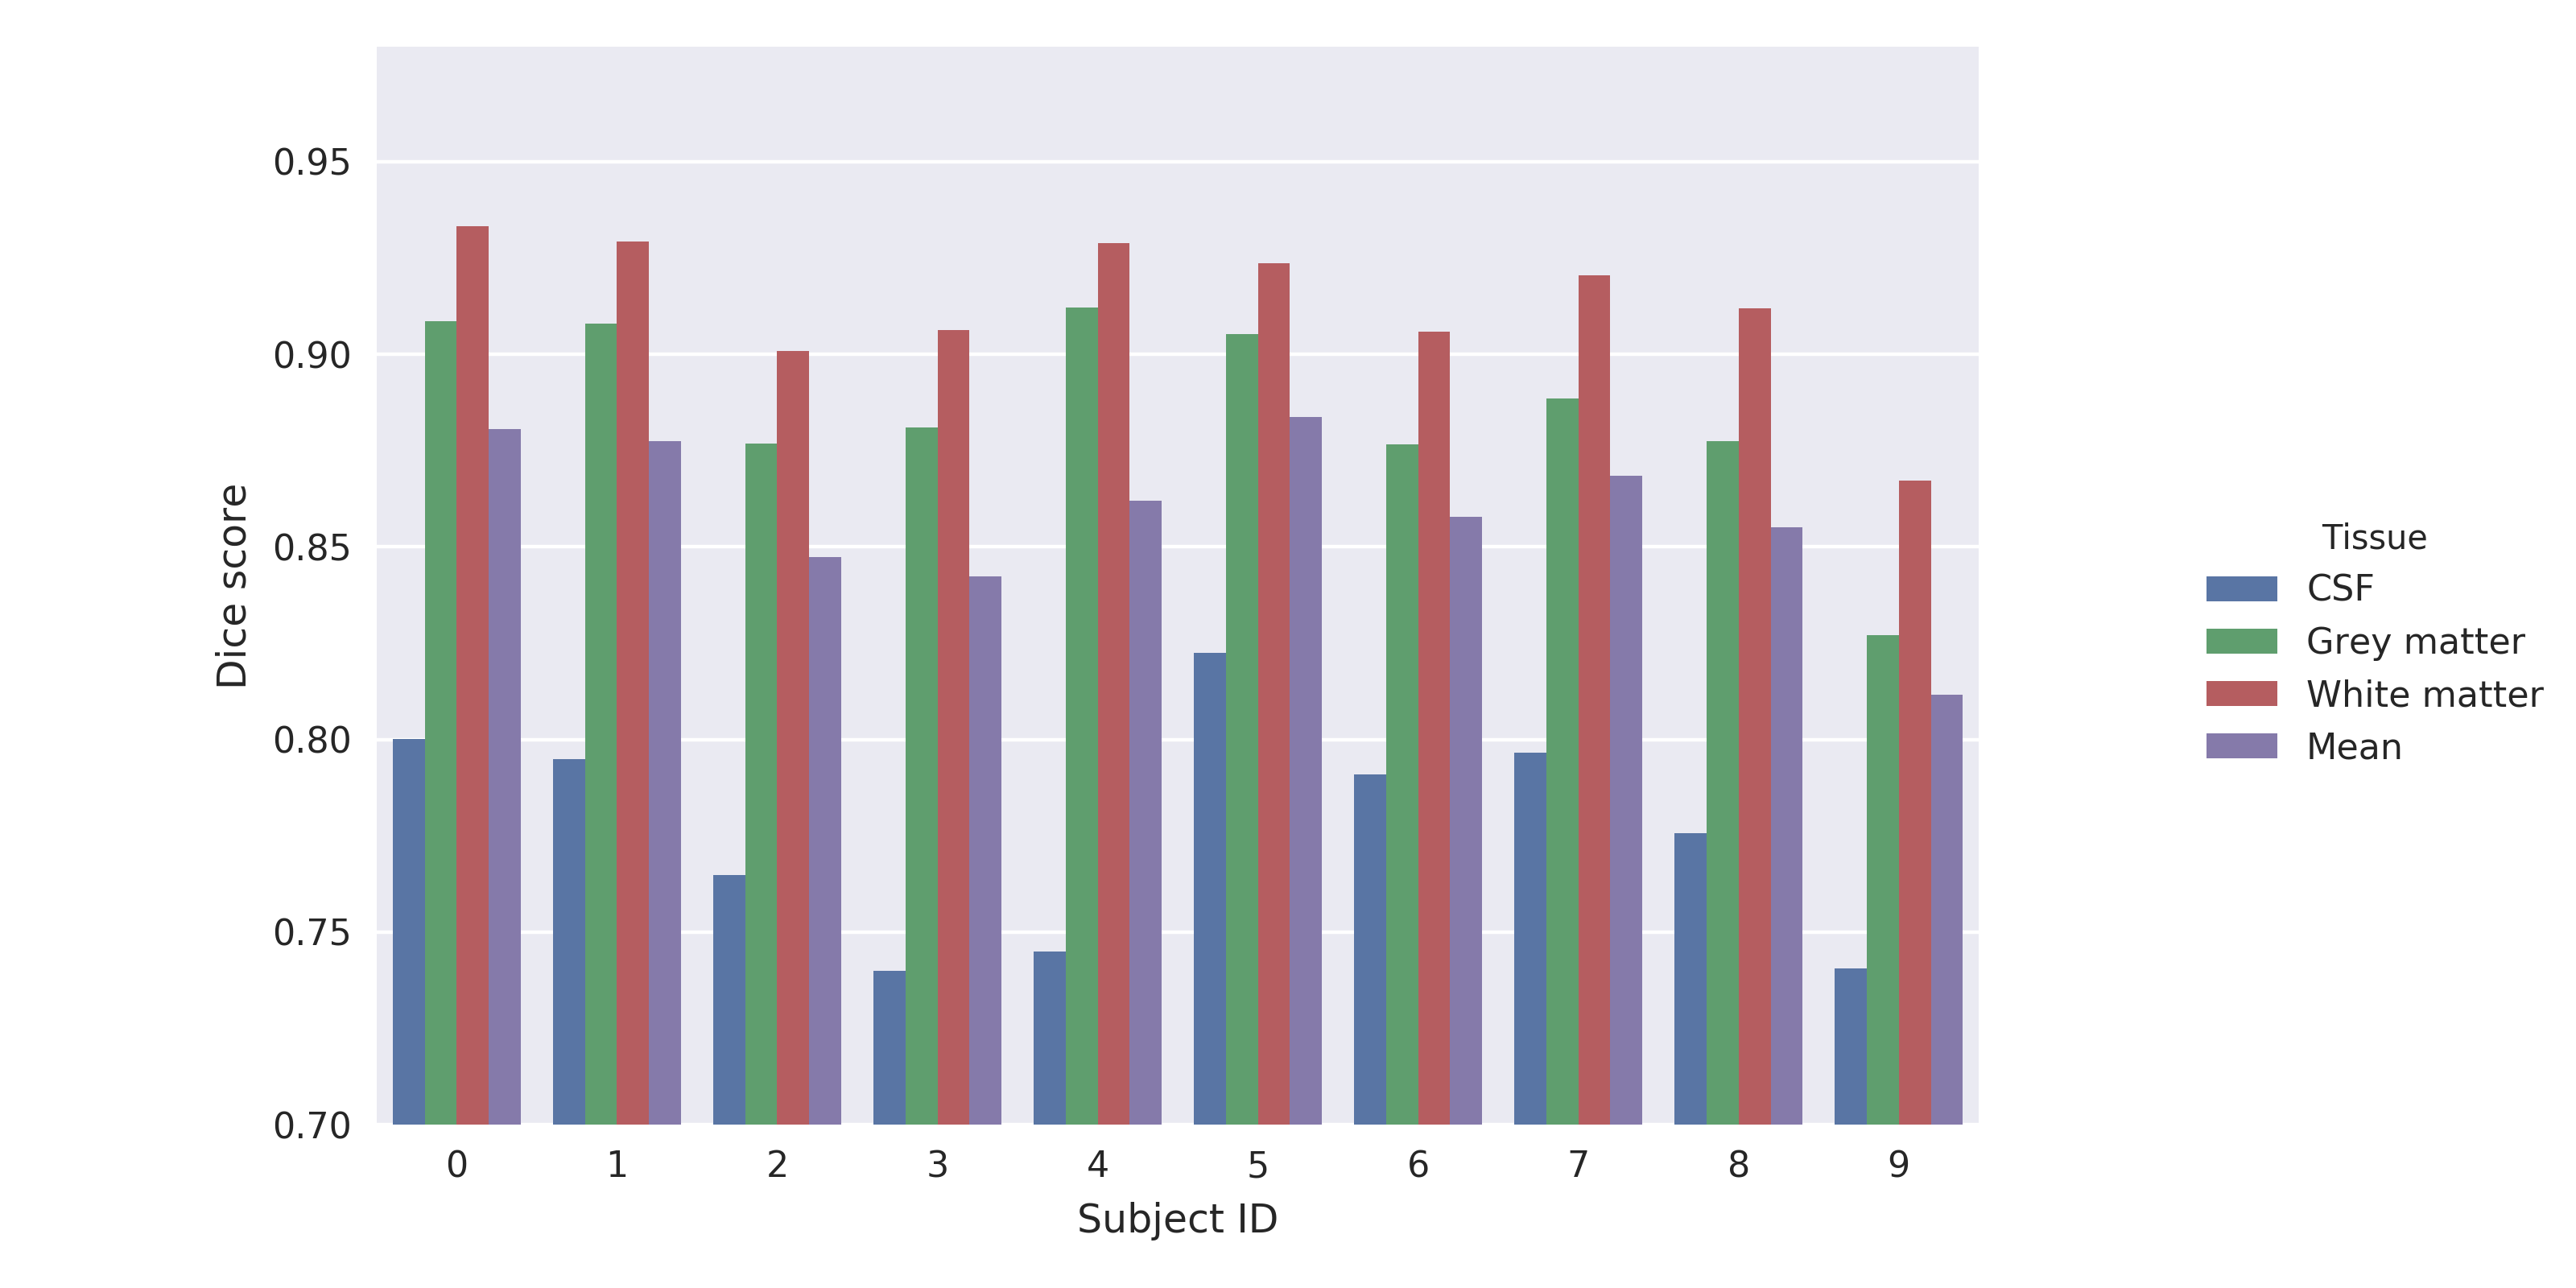
\includegraphics[width=\textwidth]{figures/dices_bars}
  \caption{Dice scores for all segmented subjects. The selected parameters seem to work best for subject 0, the one used for the optimisation. These parameters work well with subject 5 as well. Optimising the parameters using all subjects would probably lead to better results.}
  \label{fig:dices-bars}
\end{figure}

\section{Statistical Analysis}




%
% ---- Bibliography ----
%
% BibTeX users should specify bibliography style 'splncs04'.
% References will then be sorted and formatted in the correct style.
%
\bibliographystyle{splncs04}
\bibliography{references}

\end{document}
